\documentclass[svgnames,11pt]{beamer}
\input{/home/tof/Documents/Cozy/latex-include/preambule_commun.tex}
\input{/home/tof/Documents/Cozy/latex-include/preambule_beamer.tex}
%\usepackage{pgfpages} \setbeameroption{show notes on second screen=left}
\author[]{Christophe Viroulaud}
\title{Petite histoire des systèmes d'exploitation}
\date{\framebox{\textbf{SE 01}}}
%\logo{}
\institute{Terminale - NSI}

\begin{document}
\begin{frame}
\titlepage
\end{frame}
\section{UNIX}
\begin{frame}
    \frametitle{UNIX}

    \begin{center}
    \centering
    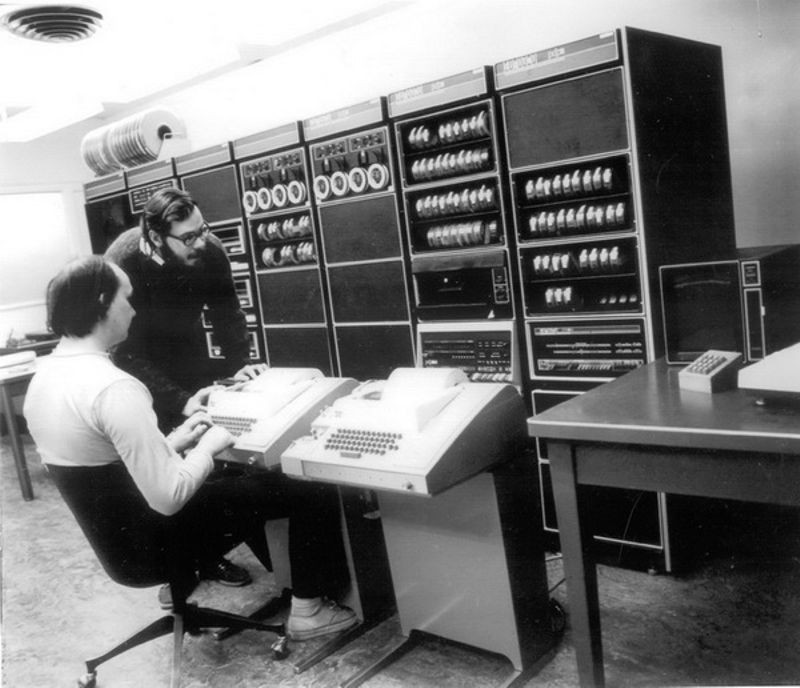
\includegraphics[width=8cm]{ressources/unix.jpg}
    \captionof{figure}{UNIX est un système d'exploitation, créé en 1969 par Ken Thompson et Dennis Ritchie.}
    \label{IMG}
    \end{center}
\note[item]{Thompson travaille chez Bell. Première système mono-utilisateur}
\note[item]{philosophie: Unix fait chaque chose d'une seule façon. Chaque utilitaire fait une seule chose mais bien}
\note[item]{Multics = système (précédant) en temps partagé}
\note[item]{création d'un nouveau langage: le C successeur du B}
\end{frame}
\begin{frame}
    \frametitle{UNIX}

\begin{aretenir}[]
Le système (et son code source) a été massivement distribué dans les universités à des fins éducatives.
\end{aretenir}
\note[item]{apparition différentes branches: BSD}
\end{frame}
\begin{frame}
    \frametitle{}

    \begin{center}
    \centering
    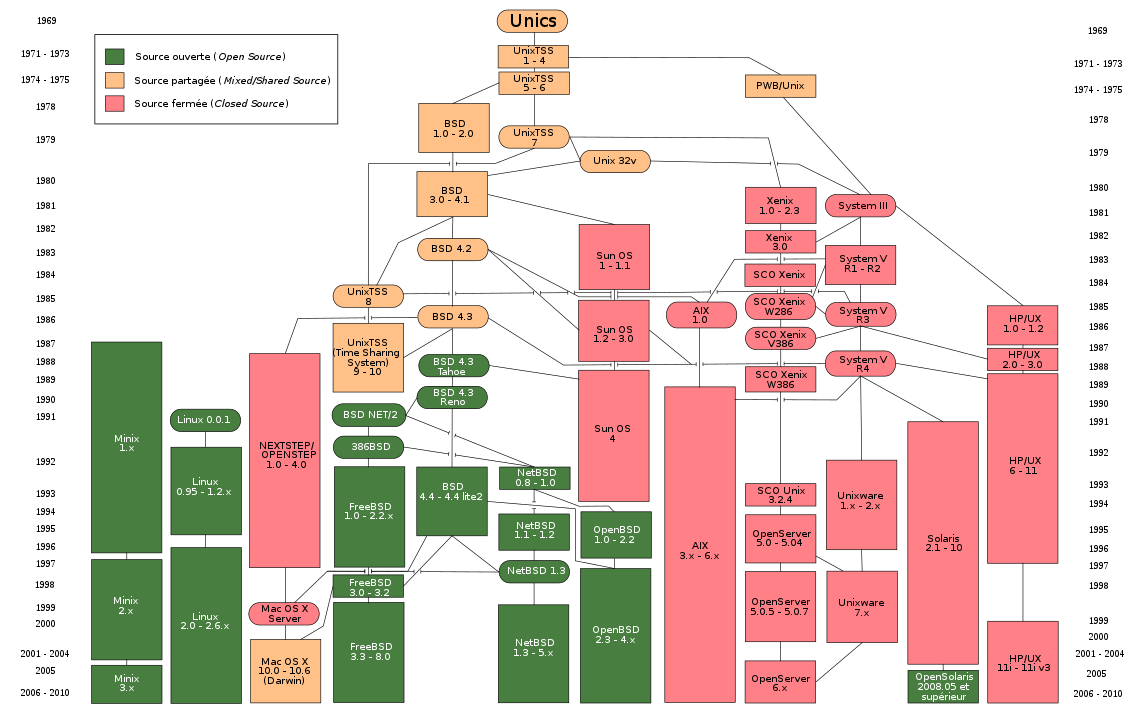
\includegraphics[width=10cm]{ressources/famille-unix.png}
    \captionof{figure}{Univers UNIX}
    \label{IMG}
    \end{center}

\end{frame}
\section{GNU}
\begin{frame}
    \frametitle{GNU}

    Scandalisé par les restrictions imposées par les logiciels propriétaires, Richard Stallman lance, en 1983, le projet GNU, qui a pour but de développer un système d'exploitation libre complet et inspiré d'UNIX, afin de contrer le développement croissant des logiciels propriétaires.
\begin{center}
\centering

\includegraphics[width=5cm]{ressources/gnu.jpg}
\captionof{figure}{Jeu de mot récursif: Gnu's Not Unix}
\label{IMG}
\end{center}
\end{frame}
\begin{frame}
    \frametitle{}
    Stallman fonde la \emph{Free Software Foundation} qui définit le logiciel libre:
    \begin{itemize}
        \item liberté d'exécution
        \item liberté de modification
        \item liberté de redistribution
        \item liberté d'amélioration
    \end{itemize}
\note{Développe la General Public License qui reprend les principes}
\end{frame}
\section{Linux}
\begin{frame}
    \frametitle{Linux}

Le noyau du système d'exploitation GNU (\emph{Hurd}) souffre d'un développement très lent. En 1991, Linus Torvalds (Finlande) développe un noyau qui est très vite adopté.
\begin{center}
\centering

\includegraphics[width=5cm]{ressources/linux.png}
\captionof{figure}{La mascotte Tux: un manchot}
\label{IMG}
\end{center}
\note[item]{très vite sous licence GPL}
\note[item]{adopté dans système GNU}
\end{frame}
\begin{frame}
    \frametitle{}

    \begin{center}
    \centering
    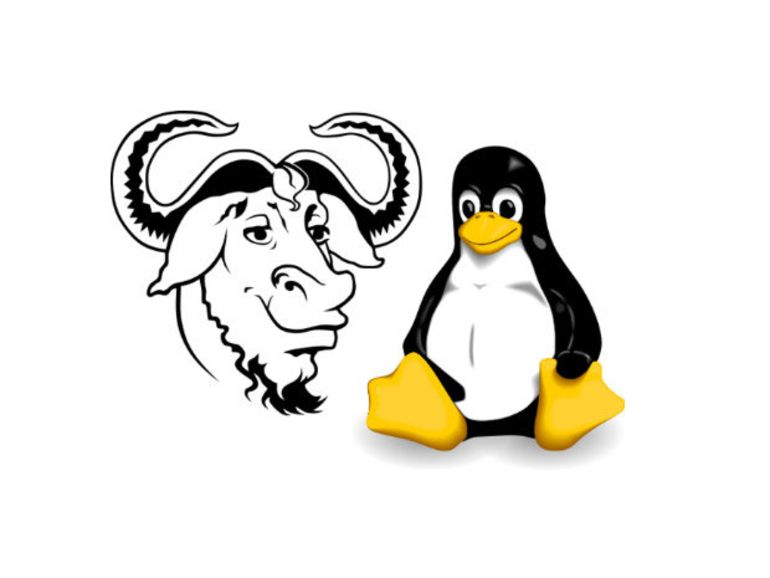
\includegraphics[width=6cm]{ressources/gnulinux.jpg}
    \captionof{figure}{De nombreuses distributions GNU/Linux}
    \label{IMG}
    \end{center}
On retrouve le noyau Linux dans de nombreuses distributions:
\begin{itemize}
    \item Debian
    \item Ubuntu
    \item Red hat
    \item Suse
\end{itemize}
\note{Modèle UNIX dans: MacOX, Android}
\end{frame}
\end{document}